\documentclass[12pt]{article}
\usepackage{sbc-template}
\usepackage[utf8]{inputenc}
\usepackage{listings}
\usepackage{xcolor}
\usepackage{textcomp}
\usepackage{graphicx}
\setlength{\parindent}{0em}


\lstdefinestyle{style1}{
    basicstyle=\ttfamily,
    columns=fullflexible,
    keepspaces=true,
    upquote=true,
}
\lstdefinestyle{style2}{
    showstringspaces=false,
    commentstyle=\color{olive},
    keywordstyle=\color{blue},
    identifierstyle=\color{violet},
    stringstyle=\color{purple},
}
\lstdefinestyle{style3}{
    language=c,
    directivestyle=\color{teal},
}
\lstdefinestyle{combined}{
    style=style1,
    style=style2,
    style=style3,
}
\lstnewenvironment{code}{
    \lstset{
        style=combined,
    }
}{}


\title{Comparando DFS e Algoritmo de Prim para detecção de ciclos em grafos não-direcionados}
\author{Rafael Amauri Diniz Augusto}
\address{PUC-MG}

\begin{document}

\maketitle

\tableofcontents
\newpage

\section{Introdução}
O algoritmo de Prim e o DFS são algoritmos que têm várias aplicações na área de estudos de grafos. 
Uma dessas aplicações é o seu uso para detecção de ciclos em grafos não-direcionados conexos, o
que vai ser melhor explorado nesse artigo e como esses algoritmos podem ser alterados para
contar o número de ciclos em um grafo simples conexo não direcionado.\vspace{10pt}

\section{Explicando os componentes do programa}


\section*{Explicando a classe Graph}


Nota: Todos os arquivos de código-fonte contém comentários e documentação extensiva. Favor
consultá-los para mais informações sobre o funcionamento do código.\vspace{10pt}


O trabalho da classe Graph é armazenar todas as informações sobre um determinado grafo, como 
a quais vértices um determinado vértice se conecta, qual o peso das arestas, o número de arestas
e o número de ciclos no grafo.\vspace{10pt}


\section*{Explicando o Algoritmo de Prim}
O algoritmo de Prim é um algoritmo guloso de complexidade O($V^2$) - com V sendo o 
número de vértices - que tem como objetivo encontrar uma Árvore Geradora Mínima(AGM)
para um determinado grafo. O seu funcionamento é escolhendo qual aresta dos vértices
já visitados tem o menor valor, e em seguida adicionando ela a um novo grafo: a 
Árvore Geradora Mínima.

Para ser usado na contagem de ciclos de um determinado grafo, o funcionamento é bem simples: como
uma AGM é um grafo conexo sem ciclos, basta substrair o número de arestas da AGM do número de
arestas do grafo padrão. Esse valor será o número de ciclos no grafo.\vspace{10pt}


\section*{Explicando o Algoritmo DFS}
O DFS é um algoritmo de travessia de grafos de complexidade O(V + E) - com V sendo o número de 
vértices e E sendo o número de arestas - se que originalmente começa a partir de um nó raiz e 
explora o grafo até onde for possível por meio de recursão.

Para ser usado na contagem de ciclos de um grafo, o DFS percorre o grafo marcando os vértices 
já visitados. Quando em um vértice V existe uma conexão para outro vértice já parcialmente
visitado, é porque existe um ciclo. Ao acumular quantas dessas conexões existem no grafo,
é encontrado o número de ciclos.\vspace{10pt}

\section{Comparação dos algoritmos e análise}
Para a comparação dos algoritmos DFS e Prim, serão usados 4 grafos conexos não-direcionados.
O tempo de execução de cada um desses algortimos será medido e comparado. A hipótese é que,
por conta da complexidade do Algoritmo de Prim ser menos eficiente que a do DFS, o algoritmo
de Prim será mais lento para achar o número de ciclos nos 4 grafos.\vspace{20pt}


\section*{Grafos}


Grafo 1:


\begin{figure}[ht]
    \centering
    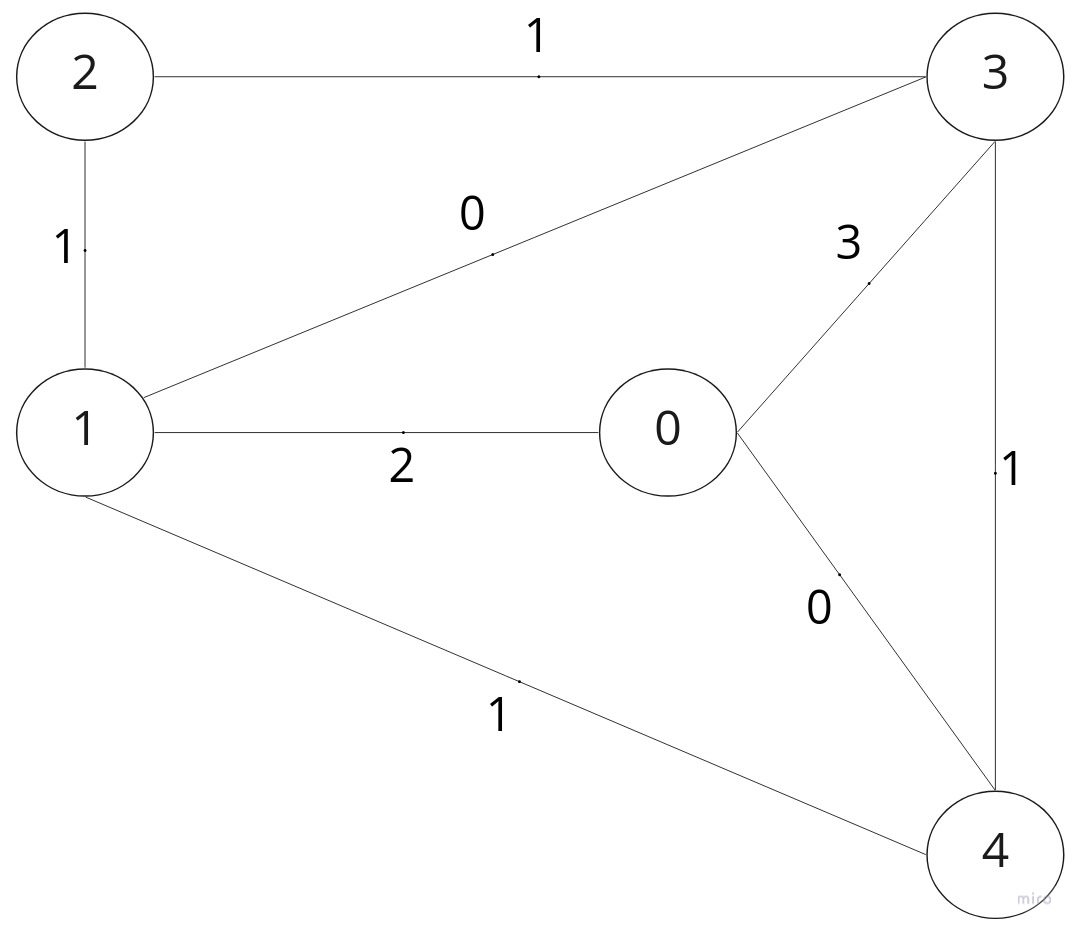
\includegraphics[scale=0.2]{grafo1.jpg}
  \end{figure}


Grafo 2:


\begin{figure}[ht]
    \centering
    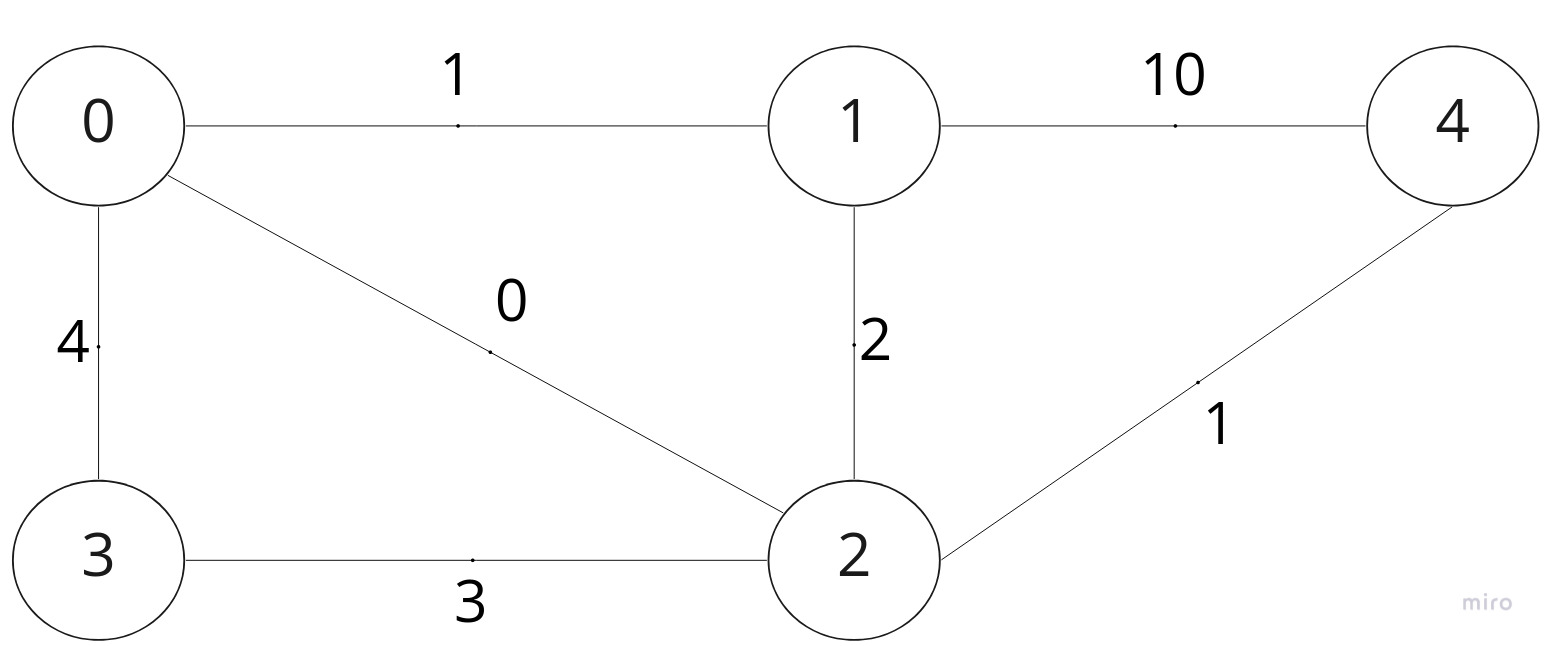
\includegraphics[scale=0.2]{grafo2.jpg}
\end{figure}

\newpage


Grafo 3:


\begin{figure}[ht]
    \centering
    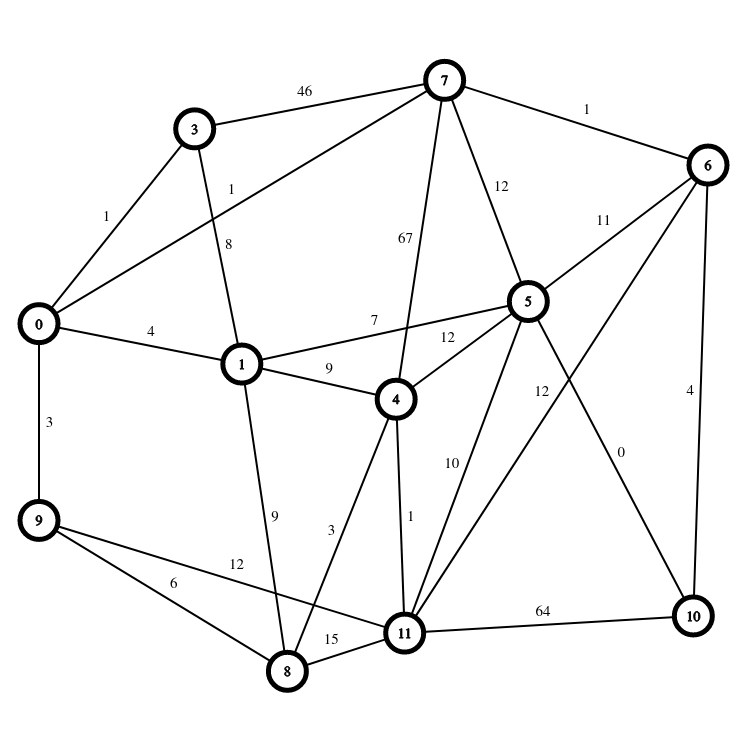
\includegraphics[scale=0.6]{grafo3.png}
\end{figure}

\newpage

Grafo 4:


\begin{figure}[ht]
    \centering
    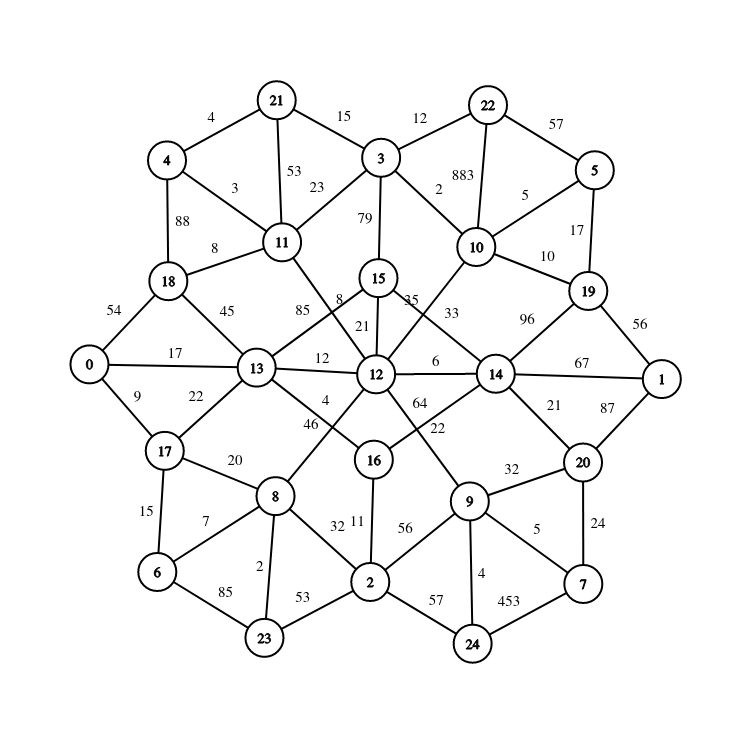
\includegraphics[scale=0.6]{grafo4.png}
\end{figure}

\newpage

\section*{Hardware}
Os testes a seguir foram efetuados em um computador com a seguinte configuração:


Sistema Operacional: Linux


Versão da kernel: 5.12.4-arch1-2


CPU: AMD Ryzen 5 5600X - 6 cores / 12 threads @ 4.6Ghz


Versão do GCC/G++: 11.1.0-1


\section*{Testes}


\begin{table}
    \begin{tabular}{lll}
    ~                           & Algoritmo de Prim          & DFS                      \\ \hline
    Complexidade                & O(V$^2$)                   & O(V + E)                 \\
    Tempo de execução - Grafo 1 & 4.15 x $10^{-5}$ segundos  & 8.87 x $10^{-6}$ segundos\\
    Tempo de execução - Grafo 2 & 3.29 x $10^{-5}$ segundos  & 6.56 x $10^{-6}$ segundos\\
    Tempo de execução - Grafo 3 & 1.92 x $10^{-3}$ segundos  & 1.82 x $10^{-5}$ segundos\\
    Tempo de execução - Grafo 4 & 5.12 x $10^{-3}$ segundos  & 7.27 x $10^{-5}$ segundos\\ 
    \end{tabular}
\end{table}


\section{Conclusões}
Como podemos ver na tabela, o Algoritmo de Prim sempre tem um tempo de execução pior que o DFS, e isso
se dá por sua complexidade ser O($V^2$), enquanto a complexidade do algoritmo DFS é O(V + E).
É notado que ambos algoritmos podem ser usados para detecção de ciclos em grafos conexos não direcionados, mas, quando performance
é levada em conta, o DFS sempre será uma alternativa melhor que o Algoritmo de Prim.


\end{document}